\documentclass[11pt, oneside]{article}  
\usepackage{geometry}                	
\geometry{a4paper}
\usepackage[parfill]{parskip}		
\usepackage{graphicx}
\usepackage{pgfgantt}
\usepackage{pgfcalendar}	
\usepackage{pgfkeys}	
\usepackage{amssymb}
\usepackage{lscape}
\usepackage{hyperref}
\hypersetup{
    colorlinks=true,
    linkcolor=blue,
    filecolor=magenta,      
    urlcolor=cyan,
}
\urlstyle{same} 

\title{COSC 345 Assignment 4} \author{Nathan Kennedy \texttt{1006384},
  Kat Lilly \texttt{8867318}, Tobyn Packer \texttt{5003352}, and
  \\Daniel Davidson \texttt{375621}} \date{\today}

\begin{document}

\maketitle
\tableofcontents
\newpage

\section{The NKTD app}

Our app now contains three functioning games which can be opened via
speech commands from the main menu and controlled either by speech
commands or through touch. Two of the games (2048 and Frozen Bubble)
are open source games we have manipulated to work with voice commands
and Teragram is an original game, a maths practice game for children.

The application uses pocketSphinx to interpret speech commands:\linebreak
\href{https://github.com/cmusphinx/pocketsphinx}{https://github.com/cmusphinx/pocketsphinx}

\subsection{Since the Beta}

We have made the following improvements and enhancements since our
beta release:

\begin{itemize}

\item Much of out codebase was refactored to have more functionality defined in RecognizedActivity to ensure consistent behaviour among its implementations

\item Much more of our code was commented to document intent in preparation for the full release

\item Bugfixes:
\begin{itemize}
	\item Fixed memory leaks upon closing Activities.
	\item Frozenbubble: Fixed launcher rotation speed.
	\item Teragram: Voice Recognition only restarts when it is
          supposed to.
\end{itemize}

\item The whole app now has a consistent design and colour scheme.

\item Modified frozen bubble launcher so that gameplay is not
  negatively impacted by the time taken inprepret commands. The
  launcher stops moving immediately on hearing a command, but waits to
  interpret it before launching the bubble, this means the delay in
  interpreting a speech command doesn't ruin the game.

\item Frozenbubble speech implementation was finished, making it
  completely playable hands-free.

\item Added an animation to the listening button, which is intuitively
  easy to understand and shows the user when the app has heard
  something or when recognition has failed.

\item Changed the way the radio buttons are labelled in multiple
  choice quizes in Teragram - we originally labelled them as ``a'',
  ``b'', ``c'' etc, but this was not suitable for voice recognition,
  so we changed it to numbers. This wasn't a satisfactory solution
  either, and we have now changed it to be labelled by colours
  instead.

\item Speech recognition stops when focus shifts from NKTD such as
  when the phone goes to sleep. It will restart when focus is returned.
\end{itemize}

\pagebreak

\section{Testing}

\subsubsection*{Voice control}

Testing an application that is run by voice commands was not something
we felt could be done through automated methods without devoting a
large amount of time that could instead be spent implementing
features. Instead, frequent testing was done manually either through
emulators or by installing the apk on our own phones. We note that the
microphone on a typical phone is significantly better than the
microphone on a typical laptop or desktop computer, and so the app is
significantly easier to play on a phone than on an emulator.

\subsubsection*{Teragram}

For the Teragram game, as well as testing it ourselves it has been
user tested by two children, seven and four years old. They still love
this game, and have still been playing it frequently.  However, they
do prefer to play it without using the voice control. This is partly
because they do not often find themselves in a quiet enough place for
the voice control to work reliably, but also because they get
frustrated that voice controls are a bit slower and less reliable than
entering answers via the touch screen. Unfortunately our app really
does work less well with voice control than touch control.

\pagebreak

\section{User Documentation}

\subsection{Common to all games}
As a user, you can say 'help me' on each of NKTD's games to bring up a
help screen displaying all speech commands available to you.
The small ear button in the bottom-right will pulse when it hears your voice 
and is going to interpret what you have said. It will shake side to side if
what it hears doesn't match a known phrase, meaning you should repeat
yourself. You can tap this button to turn speech recognition off or on.

\subsection{Teragram}

The game starts up at level one, and the user can move to the easiest
level by tapping the `too hard' button or go up levels by tapping the
`too easy' button. When ten questions in a row are answered correctly,
the game will automatically level up, otherwise if two questions are
incorrect in a row, it'll automatically level down.  The user is not
aware of the actual level, it's just that questions get easier or
harder - the bound on the random number generator used in setting new
questions is related to the level.

The game launches in addition mode, and the user can chose to move to
subtraction problems, or practice times tables or powers of two.

\subsection{2048}

2048 is a popular number name released on March 20, 2014. This game is
very simple; you can choose to slide the tiles up, down, left or right
by swipping the screen or saying `left', `right' `up' or `down'. Every
slide, all the digital squares will move in the direction the screen was slid. 
This is a really neat game, and there are many open source
implementations out there, but what makes it especially suitable for
our app is the simplicity of its controls - it's an interesting and
challenging game controlled with only four commands. Also there is no
time pressure in this game, so if it takes half a second for the
speech recogniser to work, this does not adversely affect the game
play.

\subsection{Frozen Bubble}
The aim of this game is to clear the screen by shooting the current
bubble from the launcher to its respective coloured bubbles on the
level. The launcher will automatically move from side to side. Saying `fire'/'now' or swiping up will shoot the bubble.

\subsection{Voice Controls}

You can control the game with the following voice commands:

\subsubsection{Main menu}

\begin{itemize}
  \item {\bf`Teragram'} or {\bf`game two'}  - this will take you to the game Teragram.
  \item {\bf`Twenty Fourty Eight'} or {\bf`game three'} - this will take you to the game 2048.
  \item {\bf`Frozen Bubble'} or {\bf`game four'} - this will take you to the game Frozen Bubble.
\end{itemize}

\subsubsection{Teragram}

\begin{itemize}
  \item {\bf`help me'} - Brings up help menu with available voice commands. 
  \item {\bf`harder'} - Provides a harder question. 
  \item {\bf`easier'} - Provides an easier question.
  \item {\bf`new question'} - Provides a new question of the same type
  \item {\bf`addition'} -Provides an addition question
  \item {\bf`subtraction'} - Provides a subtraction question
  \item {\bf`times tables'} - Starts times tables practice mode
  \item {\bf`powers of two'} - Starts powers of two quiz
  \begin{itemize}
  	\item Say the colour of the correct answer: {\bf`blue'}, {\bf`green'}, {\bf`pink'}, or {\bf`red'}
  \end{itemize}
  \item {\bf`number'} - Starts Number Input mode, see below
  \item {\bf`exit'} - Prompts a message confirming if they want to exit
 
\end{itemize}

\subsubsection{2048}

\begin{itemize}
  	\item {\bf`help me'} - Brings up help menu with available voice commands. 
	\item {\bf`left'} - All blocks will move to the left if possible. 
	\item {\bf`right'} - All blocks will move to the right if possible
	\item {\bf`up'} - All blocks will move to up if possible. 
	\item {\bf`down'} - All blocks will move to down if possible
	\item {\bf`exit'} - Prompts a message confirming if they want to exit
	
\end{itemize}

\subsubsection{Frozen Bubble}

\begin{itemize}
	\item {\bf`fire'} or {\bf`now'} - Will fire the bubble or proceed to the next
	level upon level completion.
	\item {\bf`exit'} - Prompts a message confirming if they want to exit
	\item {\bf`continue'} - Continues the launcher's auto-rotation after a pause.
	\item {\bf`colorblind'} - Toggles colorblind mode.
	\item {\bf`full screen'} - Toggles fullscreen mode.
	\item {\bf`(don't) rush me'} - Toggles `Rush Me' mode.
	\item {\bf`about frozen bubble'} - Displays Frozen Bubble credits. Say 'continue'
	to close it.
	\item {\bf`new game'} - Starts a new game.
	\item {\bf`help me'} - Displays a help screen.
	
\end{itemize}

\subsubsection{Number Input}
\begin{itemize}
  \item {\bf numbers 0 to 9 inclusive} – Appends the spoken number
    to the end of your answer, ie. Speaking `one', `two' will give you
    12. Note that 0 is to be spoken `zero'
  \item {\bf `okay'} - Submits the current answer and exits Number
    Input mode
  \item {\bf `back'} - Removes the last number from your answer
  \item {\bf `clear'} - Removes the entirety of your answer
  \item {\bf `cancel'} - Exits Number Input mode
\end{itemize}

When entering numbers, please wait until the number you have just spoken appears
in the box before trying to input the next one.
Good Luck!

\pagebreak

\section{Developer Documentation}

\subsection{Build Instructions}
The project can be built using Android Studio standard settings.

\subsection{Application Architecture}
The application consists of multiple RecognizedActivities that
interact with a Recognizer service with assistance from a
SpeechResultListener.

\begin{figure}[!h]
	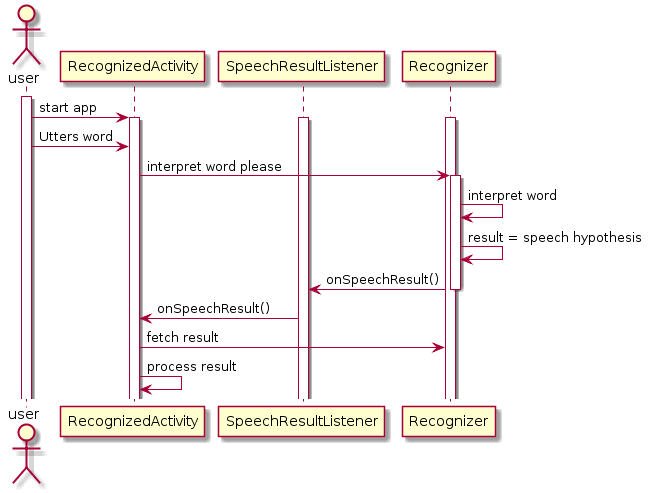
\includegraphics[width=0.7\columnwidth]{speechsequence}
	\caption{Interpreting a voice command.}
\end{figure}

\subsubsection{RecognizedActivity}
RecognizedActivity is an extension of AppCompatActivity that contains
extra functionality for keeping the Recognizer service running in the
correct mode throughout Activity switching and Dialog popups. In each implementation the method 'setup()' needs to be called in its 'onCreate()' method. Each RecognizedActivity needs to have an ImageButton in its layout with the id recognizerStatus and a listener that implements the method 'onSpeechResult()'. 'setup()' will add functionality to these for you as well as binding the Recognizer.

\subsubsection{Recognizer}
Recognizer is a Service that implements a CMUSphinx interpreter to
interpret speech from a user and use the interpretations to control a
RecognizedActivity. It is important that the Recognizer is able to
switch between different modes of search to represent the
RecognizedActivity that the user is currently interacting with. It
does this by switching between 'grammar' files written in JSpeech
Grammar Format. These files tell the interpreter what words and in
what order it should expect them.

\subsubsection{SpeechResultListener}
SpeechResultListener listens for events in the Recognizer Service and
informs the current RecognizedActivity that they have happened. It
contains code that maintains the RecognizedActivity's recognizerButton
such as swapping the image and initiating animations. The most
important method is onSpeechResult() which informs the Activity that
there is a new speech result for it to fetch. This method is abstract
and needs to be implemented in each individual Activity and should
contain code to handle each speech command the Activity can expect to
find.

\section{Open Source components}

The code for the speech recognizer setup/permissions/asset copying is
taken almost directly from the pocketSphinx demo application here:
\url{https://github.com/cmusphinx/pocketsphinx-android-demo}

The phoneme definitions in our nktd.dic file are selectively taken
from the cmudict-en-us.dict file in that same demo.

The acoustic model we use is provided by CMUSphinx at
\href{https://sourceforge.net/projects/cmusphinx/files/Acoustic\%20and\%20Language\%20Models/US\%20English/}{sourceforge.net}

The game FrozenBubble taken from
\url{https://github.com/kthakore/frozen-bubble}

The game 2048 taken from
\url{https://github.com/BuddyBuild/2048-Android}
    


\end{document}
